%
% Tesi D.S.I. - modello preso da
% Stanford University PhD thesis style -- modifications to the report style
%
%%%%%%%%%%%%%%%%%%%%%%%%%%%%%%%%%%%%%%%%%%%%%%%%%%%%%%%%%
%
%--fix template
\makeatletter
\let\my@xfloat\@xfloat
\makeatother
%--end fix
\documentclass[a4paper,12pt]{report}
%    \renewcommand{\baselinestretch}{1.6}      % interline spacing
%
% \includeonly{}
%
%			PREAMBOLO
%
\usepackage[a4paper]{geometry}
\usepackage{amssymb,amsmath,amsthm}
\usepackage{graphicx}
\graphicspath{{./img/}}
\usepackage{url}
\usepackage{hyperref}
\usepackage{epsfig}
\usepackage[italian]{babel}
\usepackage{setspace}
\usepackage{tesi}
%--definizione linguaggio
\usepackage{listings}
\usepackage{color}
\definecolor{dkgreen}{rgb}{0,0.6,0}
\definecolor{gray}{rgb}{0.5,0.5,0.5}
\definecolor{mauve}{rgb}{0.58,0,0.82}

\lstset{frame=tb,
  language=Bash,
  aboveskip=3mm,
  belowskip=3mm,
  showstringspaces=false,
  columns=flexible,
  basicstyle={\small\ttfamily},
  numbers=none,
  numberstyle=\tiny\color{gray},
  keywordstyle=\color{blue},
  commentstyle=\color{dkgreen},
  stringstyle=\color{mauve},
  breaklines=true,
  breakatwhitespace=true,
  tabsize=3
}
%--fine definizione linguaggio

%--fix template
\makeatletter
\def\@xfloat#1[#2]{
	\my@xfloat#1[#2]%
	\def\baselinestretch{1}%
	\@normalsize \normalsize
}
\makeatother
%--end fix



% per le accentate
\usepackage[utf8]{inputenc}
%
\newtheorem{myteor}{Teorema}[section]
%
\newenvironment{teor}{\begin{myteor}\sl}{\end{myteor}}
%
%
%			TITOLO
%
\begin{document}
\begin{center}

\includegraphics[width=\textwidth]{Logo.jpg}
\title{Realizzazione di una soluzione IAC (Infrastructure As Code) che consenta il rilascio di un'infrastruttura per ambiti DevOps}
\end{center}
\author{\textbf{Roberto Antoniello}}
\dept{Corso di Laurea in Informatica} 
\anno{2022-2023}
\matricola{\textbf{875693}}
\relatore{Prof. Valentina Ciriani}
\correlatore{Mario Petrella}

\beforepreface

\afterpreface
% 
% 
% 
\chapter{Introduzione}
\section{IAC: definizione e vantaggi}
La metodologia IAC(Infrastructure As Code), in italiano "infrastruttura come codice", è una strategia che punta a gestire l'intero ciclo di vita di un'infrastruttura mediante codice. Quindi non c'è bisogno di configurazione hardware fisica o strumenti interattivi esterni, è sufficiente uno o più linguaggi dichiarativi o di scripting e compilare correttamente dei file di definizione.\cite{iacdef} \\ 
In questo modo è molto più semplice e rapido modificare o eseguire miglioramenti al sistema senza dover ripensare completamente la struttura o stravolgerne le componenti. \\
Come vedremo nei successivi paragrafi, la potenza di alcune delle tecnologie trattate lungo lo sviluppo di questo progetto risiede proprio nel fatto di poter essere gestite direttamente tramite codice.\\
In questo capitolo introduttivo saranno descritti gli obiettivi prefissati per questo progetto, le fasi principali che sono state svolte e una breve descrizione delle tecnologie utilizzate. \\
In questo modo sarà più immediato richiamare alcuni concetti che useremo nei capitoli successivi.
\section{Obiettivi del progetto}
Gli obiettivi principali prefissati per questo progetto di tirocinio sono stati i seguenti:
\begin{enumerate}
\item \textit{Acquisire competenze in ambito DevOps.}
\item \textit{Acquisire conoscenze sul ciclo di vita di un'infrastruttura.}
\item \textit{Costruire un'infrastruttura in grado di essere rilasciata attraverso il cloud e sulla quale fosse possibile rilasciare applicazioni basate su microservizi.}
\end{enumerate}
\subsection{Dal metodo tradizionale all'approccio DevOps}
DevOps è una metodologia che punta a ridurre in modo considerevole i tempi di rilascio di nuovo software incorporando nello stesso di team di sviluppo le competenze necessarie per costruire l'infrastruttura adatta al rilascio del software grazie ai concetti di container, microservizi e cloud computing.\\
Tradizionalmente il processo di rilascio avveniva più lentamente nell'arco di mesi. Il team di sviluppo doveva coordinarsi con gli altri team per le diverse fasi dello sviluppo. Oggi invece con lo sviluppo DevOps si possono eseguire tutte le fasi senza dover aspettare un team separato, garantendo che il tempo di rilascio delle modifiche del software possa avvenire con frequenza oraria o anche meno, oltre ad essere continuativo e automatico.\\
Un'ulteriore progresso in questo tipo di approcci è il DevSecOps, una strategia che va a integrare anche la sicurezza e il testing nel CI(Continuous Integration) e CD(Continuous Deployment). \\La difficoltà che sorge nel DevSecOps è la risoluzione dei problemi legati alla sicurezza internamente al team di sviluppo, poichè gli sviluppatori devono prima acquisire le competenze necessarie per risolvere questo tipo di problemi.
\subsection{Ciclo di vita dell'infrastruttura}
Si intende in tal senso che l'obiettivo specifico fosse di comprendere l'intero ciclo a partire dall'analisi dei requisiti fino ad arrivare alla progettazione e implementazione finale del sistema.
\section{Fasi principali svolte}
Le principali fasi svolte durante il progetto di tirocinio sono state le seguenti:
\begin{enumerate}
\item \textit{Studio delle tecnologie coinvolte.} \\
Durante questa fase sono state approcciate diverse tecnologie per la prima volta. Vi è stato un primo apprendimento teorico dei concetti che ruotavano attorno al funzionamento di questi strumenti, mentre successivamente tali concetti sono stati applicati in maniera pratica eseguendo diversi test.
\item \textit{Progettazione dell'infrastruttura.} \\
In questa fase è stata eseguita un'analisi dei requisiti e definita la struttura dell'infrastruttura finale. Per fare ciò è stata sfruttata la fase iniziale di studio per capire in che modo le varie tecnologie andassero collegate tra loro in maniera corretta.
\item \textit{Implementazione del sistema.}\\
In questa fase finale è stata implementata l'infrastruttura in funzione dei disegni progettuali prodotti in precedenza.\\
Una volta costruito il sistema e quindi l'ambiente operativo di base, è stata poi rilasciata al suo interno un'applicazione a microservizi. \\
Come da requisiti iniziali anche le successive modifiche all'applicazione potevano avvenire in automatico in regola con la CI/CD. \\
\end{enumerate}

\section{Tecnologie utilizzate}
\begin{figure}[h]
	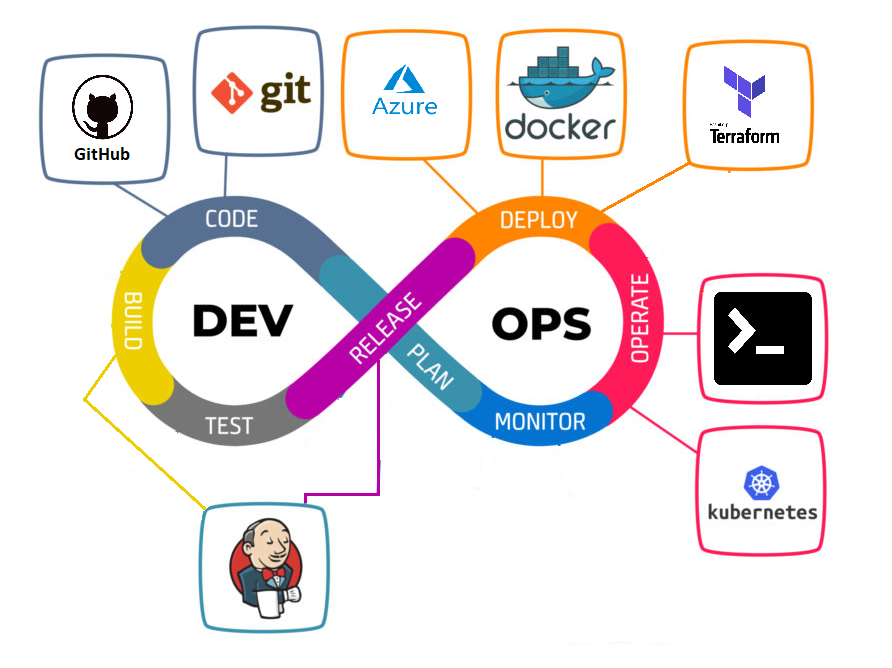
\includegraphics[width=0.6\textwidth]{tech_used}
    \caption{The DevOps infinity loop(ogni tecnologia utilizzata nel proprio settore) \cite{devopsloopimg}}
    \label{fig:tech_used}
\end{figure}
In questa figura è possibile osservare l'elenco delle tecnologie utilizzate, ognuna posta nel proprio settore di appartenenza lungo il ciclo infinito dello sviluppo DevOps.\cite{devopsloop}\\
Questo ciclo parte dalla stesura del codice fino ad arrivare al suo monitoraggio per poi ricominciare da capo senza mai concludersi.\\
Per quanto riguarda il versionamento del codice è stato utilizzato \textbf{Git}. \\
Spostandoci sul lato del deploy notiamo \textbf{Azure} che è il cloud provider scelto durante la fase di studio, \textbf{Terraform} per la vera e propria infrastruttura a livello di codice e \textbf{Docker} per la sua funzionalità nella creazione di container.\\
Potremo invece considerare \textbf{Kubernetes}  come il "controller" di tutto il sistema costruito durante il progetto.\\
Infine per la parte di build e release è stato utilizzato \textbf{Jenkins} per tutto ciò che riguarda il continuo rilascio in maniera automatica.\\
\textit{Nel prossimo capitolo andremo ad approfondire meglio i concetti principali di queste tecnologie e come sono state utilizzate nel contesto del progetto.}

%-------------------------------------------------

\chapter{Fase di studio e analisi dei requisiti}
\section{Tecnologie}
Come anticipato, in questa sezione si parlerà più nel dettaglio delle tecnologie già menzionate e più nel dettaglio della fase di studio.
\subsection{Docker}
Docker è un software progettato per permettere di eseguire applicazioni in ambienti isolati minimali e facilmente distribuibili, anche detti container. \cite{docker} \\
Andando più nel dettaglio questi container non sono altro che delle applicazioni "virtualizzate" ma che condividono il kernel del sistema operativo della macchina che li ospita. \\
Nel contesto del progetto Docker è stato usato direttamente solo per il versionamento delle immagini dei microservizi. È stato invece usato in modo implicito e indiretto all'interno di Kubernetes.
\subsection{Kubernetes}
Kubernetes, anche chiamata k8s, è una piattaforma open source che automatizza le operazioni sui container. Grazie ad essa vengono eliminati molti dei processi manuali coinvolti nel deploy di applicazioni in container. \\
Non è più necessario manipolare i container a mano con diversi comandi Docker, ma è sufficiente scrivere un manifesto in codice formato YAML. In questo file vengono definite le specifiche del container e ogni volta che dovrà essere modificato basterà modificare il codice e successivamente applicare di nuovo il file. \\
È possibile mettere in cluster gruppi di nodi su cui sono in esecuzioni dei container e Kubernetes aiuta a gestirli in modo facile ed efficiente.\\
Questa tecnologia si pone a un livello d'astrazione più alto rispetto a Docker e i nodi all'interno del cluster contengono già al loro interno un container runtime.\cite{kubernetes}\\ \\

\subsection{Azure}
Nel corso della fase di studio, tra le varie alternative possibili è stato scelto Azure come cloud provider su cui fare affidamento.\\
I vantaggi di usare il cloud risiedono nel fatto che non è più necessario costruirsi un proprio datacenter privato acquistando hardware e gestendolo privatamente, ma noleggiandolo da società terze sfruttando la rete.\cite{cloud}\\
L'utilizzo delle macchine è pagato sulla base dell'effettivo consumo e come detto poc'anzi questo fa si che i costi da sostenere siano notevolmente più bassi rispetto all'acquisto, installazione e manutenzione in loco.\\
Nel contesto del progetto Azure è stato usato principalmente per il suo servizio legato ai cluster Kubernetes, chiamato Azure Kubernetes Service o in forma abbreviata AKS. Oltre alla convenienza sul lato economico, un vantaggio in questo caso specifico sta nel ritrovarsi con un cluster già pronto e operativo con un singolo comando dalla CLI di Azure o con pochi click dal portale web.\\
Alternativamente, se dovessimo fare a meno di questo servizio, saremmo costretti a configurare a mano le diverse macchine per collegarle insieme e formare il cluster. 
\begin{lstlisting}[caption={\\\textit{Esempio di comando per creare un cluster Kubernetes come servizio di Azure da Azure CLI. Gli argomenti passati sono il gruppo risorse in cui deployare la risorsa di tipo AKS, il nome attribuito al cluster e il numero di nodi desiderati.}}]
az aks create \
  --resource-group <gruppo-risorse> \
  --name <nome-cluster> \
  --node-count <n> \
\end{lstlisting}

\subsection{Terraform}
Si tratta di una tecnologia di automazione dotata di un proprio linguaggio dichiarativo HCL(Hashicorp Configuration Language), con la quale è possibile creare, modificare e eventualmente distruggere risorse descritte nel codice.\\
Nel contesto del progetto Terraform è stato utilizzato per definire le specifiche del cluster Kubernetes come servizio di Azure. Una volta che è stato definito tramite codice, non è stato più necessario andarlo a creare attraverso Azure stesso, ma semplicemente facendo compilare e applicare il codice.
\subsection{Jenkins}
Questo è stato uno strumento fondamentale ai fini del progetto, nonché ponte di collegamento tra tutte le tecnologie introdotte finora. \\
È un software open source di supporto allo sviluppo che permette facilmente l'integrazione continua e automatica nei rilasci del software.\cite{jenkins}\\
Jenkins è stato utilizzato in questo progetto per costruire delle cosiddette pipeline, ovvero delle collezioni di eventi che succedono uno dopo l'altro. Andando più nel dettaglio, ogni pipeline prodotta è divisa in diversi blocchi, ognuno dei quali esegue determinate azioni tramite un apposito script in Bash.\\
Ogni qualvolta viene fatta una modifica, una pipeline specifica viene attivata ed eseguita dall'inizio fino alla fine, il tutto in autonomia e senza bisogno di passi manuali.
\section{Requisiti}

\subsection{collegamenti tra le tecnologie}

\chapter{Progettazione dell'infrastruttura}
\section{Casi d'uso}
\section{Definizione dell'infrastruttura}
\subsection{Ulteriori dettagli progettuali}

\chapter{Implementazione in funzione dei disegni progettuali}
\section{Codice Terraform e pipeline dedicata}
\subsection{Definizione via codice}
\subsection{pipeline per la gestione delle modifiche}
\section{Sviluppo pipeline per il rilascio dei micro servizi e modifica di puntamenti nel sorgente}
\subsection{Definizione delle pipeline}
\subsection{Modifica nel codice sorgente}

\chapter{Conclusioni: risultati raggiunti e possibili miglioramenti}
\section{risultati raggiunti al termine}
\section{miglioramenti}

%
%			BIBLIOGRAFIA
%
\begin{thebibliography}{00}
%
\bibitem{iacdef}
Wikipedia, Infrastructure As Code. \url{https://it.wikipedia.org/wiki/Infrastructure_as_Code}

\bibitem{devopsloopimg}
Shalb.com, What is DevOps and where is it applied? 2019.\url{https://shalb.com/blog/what-is-devops-and-where-is-it-applied/}

\bibitem{devopsloop}
TechTarget, Demystify the DevOps process, step by step, 2023. \url{https://www.techtarget.com/searchitoperations/tip/Demystify-the-DevOps-process-step-by-step}

\bibitem{docker}
Wikipedia, Docker. \url{https://it.wikipedia.org/wiki/Docker#Orchestrazione}

\bibitem{kubernetes}
Wikipedia, Kubernetes. \url{https://it.wikipedia.org/wiki/Kubernetes}

\bibitem{cloud}
Ionos.it, I vantaggi del cloud computing. 2023 \url{https://www.ionos.it/digitalguide/server/know-how/i-vantaggi-del-cloud-computing/}

\bibitem{jenkins}
Wikipedia, Jenkins. \url{https://it.wikipedia.org/wiki/Jenkins_(software)}
%
%
\end{thebibliography}
% 
\end{document}


 
